\chapter{Estado del arte} \label{sec:capítulo_2}

\section{Organización de los datos}

Aunque es común emplear sistemas de ficheros para organizar los datos, desde un punto de vista técnico, es posible almacenarlos sin una estructura específica en un disco. Aunque este enfoque es poco común, plantea desafíos en términos de organización y eficiencia. Para comprender mejor cómo organizar datos, resulta esencial entender la disposición física en diversos medios de almacenamiento y sus estructuras inherentes.

\subsection{Organización física de los datos en el disco}

La organización física de los datos en discos es crucial para garantizar la precisión en la organización y la efectividad en la gestión de la información, siendo los discos duros (HDD) y las unidades de estado sólido (SSD) los medios de almacenamiento más comunes en la actualidad. Esta estructura subyacente, invariable ante el sistema de ficheros utilizado, establece los cimientos para un acceso rápido y fiable a los datos, independientemente del medio de almacenamiento empleado.\\

En el núcleo de un disco duro magnético, nos encontramos con platos magnéticos concéntricos; cada uno con dos caras utilizables para el almacenamiento. Estas caras se convierten en unidades de almacenamiento independientes, y un cabezal de lectura/escritura flota sobre la superficie del plato para acceder y modificar los datos. En la actualidad, tenemos como alternativa a los discos magnéticos los denominados discos de estado sólido, que difieren significativamente de los discos duros tradicionales\cite{Hdd}.\\
 
Los discos de estado sólido se caracterizan por prescindir de partes móviles, optando en su lugar por tecnología flash para el almacenamiento. Esto se traduce en un acceso aleatorio considerablemente más rápido. Por ejemplo, la velocidad de acceso aleatorio típica de una unidad de estado sólido puede ser de alrededor de 0.1 milisegundos o incluso menos, mientras que la velocidad de acceso de un disco duro magnético convencional generalmente oscila en el rango de milisegundos, siendo normalmente más lenta.\\ 

Cabe destacar que, a pesar de que los discos de estado sólido superan en velocidad a los discos duros magnéticos, todavía se sitúan por debajo de la velocidad de acceso a la memoria principal, que es del orden de 0.1 microsegundos\cite{InsideSolidState}.

Para ambos tipos de discos, el sistema operativo tiene una visión lógica del disco como una tira secuencial numerada de bloques. Para leer o escribir en un bloque, el sistema operativo solo necesita identificar el dispositivo y el número de bloque correspondiente. Sin embargo, el controlador de disco gestiona la información de manera más cercana al hardware. 

\begin{figure}[h!]
    \centering
    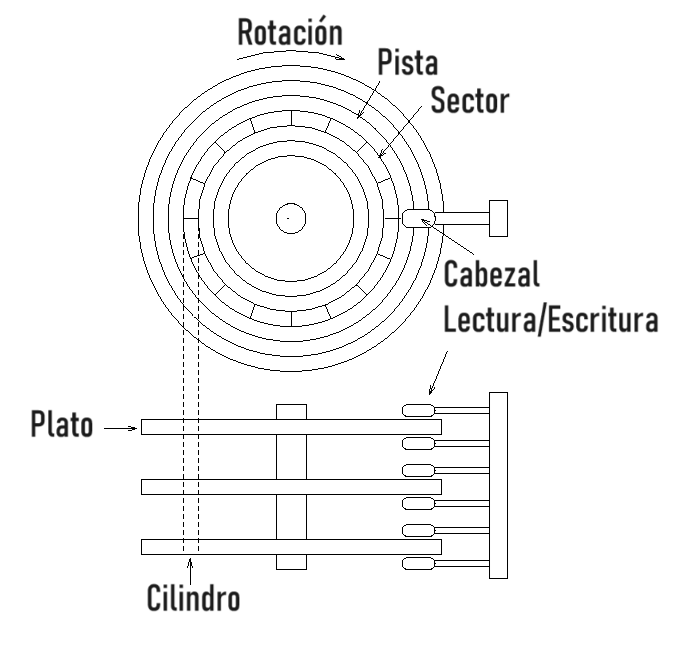
\includegraphics[width=0.75\linewidth]{figures/disk_platters.png}
    \caption{Estructura física de un disco mecánico}
    \label{fig:estructura_fisica_disco_mecanico}
\end{figure}

En el caso de los discos mecánicos, como podemos ver en la figura \ref{fig:estructura_fisica_disco_mecanico}, el controlador de disco utiliza ternas de números (número de cilindro, número de pista y número de sector) para gestionar la información del disco. Cada bloque de datos en el sistema de ficheros corresponde a varios sectores físicos del disco. La numeración de los sectores (bloques) sigue un criterio que favorece los accesos secuenciales \cite{Hdd}.\\

A nivel físico, se establece un factor de intercalación que permite resolver el problema de perder uno o varios sectores por efecto de la velocidad de rotación mientras estamos completando la transferencia interna de datos entre la controladora y el sistema operativo. Con ello, se reduce el número de rotaciones necesarias para leer, por ejemplo, una pista completa secuencialmente \cite{StorageSystems,valero2006}.\\

Por otro lado, en el caso de los discos de estado sólido, la organización física es diferente debido a la ausencia de partes móviles. En lugar de acceder a los datos a través de cilindros, pistas y sectores como en los discos duros mecánicos, en los discos de estado sólido los datos se almacenan y acceden de manera electrónica directamente en las celdas de memoria flash \cite{InsideSolidState}.

\subsection{Organización lógica de los datos en el disco}

Independientemente de la organización física que puedan presentar, la gran mayoría de los sistemas de ficheros de Unix siguen una estructura lógica fundamental para gestionar y acceder a los datos almacenados en el disco. Esta estructura lógica, presente en sistemas de ficheros tanto en discos duros mecánicos como en unidades de estado sólido, permite una gestión eficiente de los datos y una fácil navegación a través del sistema de ficheros \cite{valero2006, linuxstorage}.

\begin{figure}[h!]
    \centering
    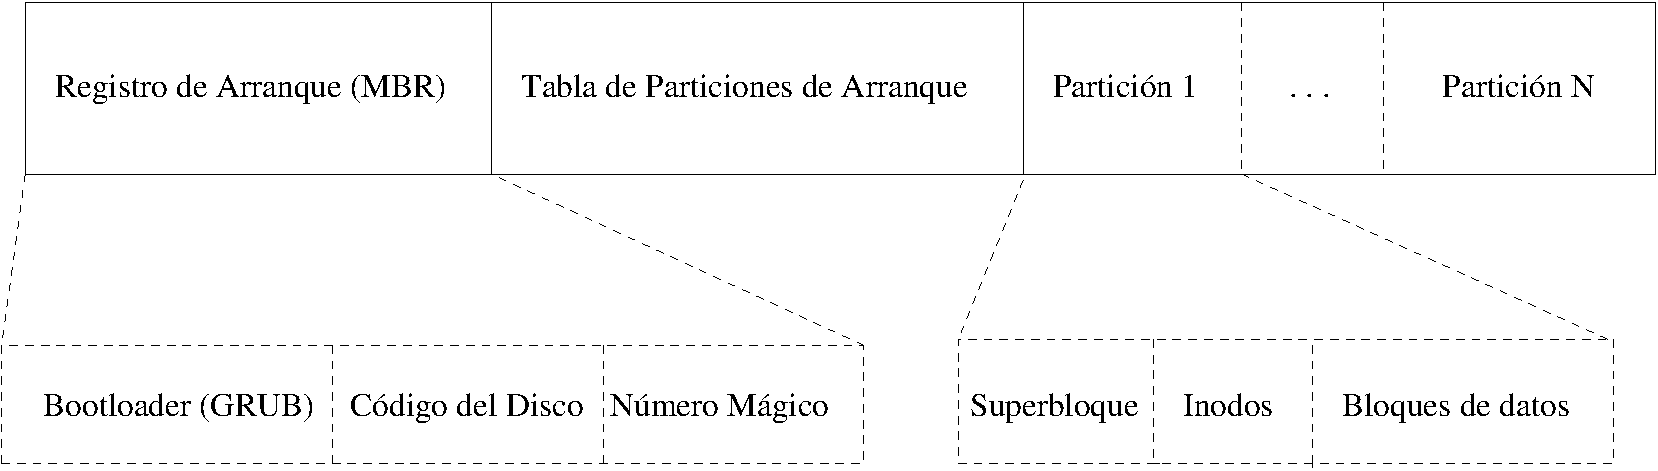
\includegraphics[width=1\linewidth]{figures/disk_logical_layout.pdf}
    \caption{Organización lógica de un disco}
    \label{fig:organizacion_logica_disco}
\end{figure}

En la figura \ref{fig:organizacion_logica_disco} se muestra la organización lógica de un disco en un sistema de ficheros tradicional, donde podemos observar las siguientes partes:

\subsubsection{MBR (master boot record)}

El MBR ocupa el primer sector o bloque del disco y contiene información esencial para el arranque del sistema y la gestión de las particiones del disco \cite{valero2006}.

\begin{itemize}
    \item \textbf{Bootloader:} El MBR almacena un programa de arranque, conocido como bootloader, que se encuentra en la primera etapa del proceso de arranque (bootstrap). El bootloader tiene la tarea de cargar el sistema operativo desde el disco y transferir el control al kernel del sistema operativo.
    
    \item \textbf{Código del disco:} Además del bootloader, el MBR puede contener código específico del disco que ayuda en el proceso de arranque, como rutinas de inicialización del hardware o controladores de dispositivo necesarios para acceder al disco y cargar el sistema operativo.
    
    \item \textbf{Número mágico:} El MBR finaliza con un número mágico de 2 bytes (0x55AA), conocido como firma de finalización, que indica que el MBR es válido y puede ser utilizado para arrancar el sistema. La presencia de esta firma es verificada por el firmware del sistema durante el proceso de arranque para determinar si el disco es arrancable. Este número mágico ha sido añadido recientemente para evitar ataques de tipo bootkit.
\end{itemize}

\subsubsection{Tabla de particiones de arranque}

La tabla de particiones de arranque, también conocida como la tabla de particiones MBR, se encuentra dentro del master boot record y describe cómo está dividido físicamente el disco en particiones. Actualmente, la tabla de particiones GPT (GUID Partition Table) es la más utilizada, ofreciendo mayor flexibilidad y soporte para discos de mayor tamaño.

\subsubsection{Particiones}

Las particiones son divisiones lógicas del disco y pueden contener diferentes sistemas de ficheros. En los sistemas de ficheros tipo Unix, cada partición suele presentar la estructura siguiente:
\begin{itemize}
    \item \textbf{Superbloque:} El superbloque es una estructura de datos crítica que se suele encontrar al inicio de un sistema de ficheros y contiene metadatos esenciales para el funcionamiento del mismo, como el tamaño total del sistema de ficheros, el tamaño de los bloques, el número de bloques libres, la ubicación de los inodos y la integridad de la partición. Es fundamental para el montaje y el mantenimiento del sistema.
    
    \item \textbf{Inodos:} Los inodos son estructuras de datos que contienen los atributos de los archivos, directorios y pipes del sistema de ficheros, cada uno de los cuales tiene asociado un inodo. Entre estos atributos se encuentra el identificador numérico del propietario (UID), del grupo de usuarios propietario (GID), máscara UGO de derechos, tamaño y ubicación en el conjunto de bloques de datos.
    
    \item \textbf{Bloques de datos:} En la parte final de la partición y ocupando la mayor parte de los bloques de la misma, se encuentran los bloques de datos, que contienen los bloques con el contenido de los ficheros, directorios y pipes. Los datos de los archivos se dividen en bloques de tamaño fijo o variable, y los inodos contienen punteros a estos bloques para acceder al contenido de los mismos.
\end{itemize}

\section{Sistema de ficheros en Linux: un análisis del sistema de ficheros virtual}

Entre otras cosas, el éxito de los sistemas Linux reside en su capacidad para interactuar sin inconvenientes con diversos sistemas de todo tipo. Esta capacidad se manifiesta en la posibilidad de montar discos o particiones que albergan formatos de fichero propios de sistemas como Windows, otros sistemas Unix e incluso sistemas como Amiga. Este destacado logro se sustenta en la implementación del innovador sistema de ficheros virtual (VFS). 

\subsubsection{El sistema de ficheros virtual}

El VFS constituye una pieza angular que opera como una capa de abstracción en el núcleo de Linux, gestionando todas las llamadas al sistema asociadas con el sistema de ficheros estándar de Unix. Su función principal consiste en proporcionar una interfaz unificada para distintos tipos de sistemas de ficheros.\\

Así, el sistema de ficheros virtual ofrece un amplio juego de llamadas al núcleo para la gestión de ficheros, las cuales son utilizadas para cualquiera de los tipos de sistemas de ficheros soportados por Linux. Cada una de estas llamadas tendrá en su implementación una parte común, es decir, ejecutada sea cual sea el sistema de ficheros subyacente, y una parte específica, que solo se ejecutará para el tipo concreto de sistema de ficheros con el que estemos trabajando en ese momento \cite{bovet2005,valero2006,bach1987}.

\subsubsection{Diversidad de sistemas de ficheros}

Los diferentes tipos de sistemas de ficheros soportados por el VFS pueden clasificarse en tres grandes grupos:

\begin{itemize}
    \item \textbf{Sistemas de ficheros basados en disco:} Son aquellos sistemas de ficheros que almacenan la información localmente en dispositivos de almacenamiento secundario (HDD, SSD, discos ópticos, memoria flash, etc).
    \item \textbf{Sistemas de ficheros en red:} Permiten el acceso a ficheros que se encuentran en otras computadoras en red. 
    \item \textbf{Sistemas de ficheros especiales:} Estos sistemas no gestionan espacio de almacenamiento real en disco, sino que actúan como interfaz con el sistema operativo para obtener o modificar información del mismo o de la configuración hardware. Un ejemplo es el sistema de ficheros \textit{/proc} en Linux.
\end{itemize}

El sistema de ficheros virtual introduce un modelo unificado para la gestión de archivos, lo que permite administrar todos los sistemas de ficheros compatibles. Por ejemplo, desde un sistema operativo Linux, un sistema de ficheros como NTFS (utilizado en Windows) se verá con una interfaz idéntica a la de Linux, incluyendo información sobre propietario, grupo y permisos UGO, adaptando las características específicas de cada sistema de ficheros al formato Unix de manera transparente \cite{love2010,tanenbaum2014}.

\section{Características principales de los sistemas de ficheros}\label{sec:caracteristicas_principales_sistemas_ficheros}

Después de examinar la organización de datos y comprender el funcionamiento del sistema de ficheros virtual, nos adentraremos en las características distintivas de los sistemas de ficheros de Linux. Exploraremos los elementos que los hacen únicos y los mecanismos implementados por el sistema para optimizar su rendimiento.

\subsection{Cachés del sistema} 

Los cachés, aunque son implementadas por el sistema operativo, desempeñan un papel crucial en los sistemas de ficheros y en las operaciones que estos realizan en el disco, así como en su rendimiento general. Por esta razón, es importante destacar los cachés más básicos que se encuentran en los sistemas actuales \cite{valero2006,bovet2005}.


\begin{figure}[!ht]
    \centering
    % TODO: falta la imagen original de esta figura en el repositorio
    % ("Screenshot 2024-02-06 at 23-12-08 ... .pdf.png"). Sustituir este
    % recuadro por \includegraphics cuando se recupere el archivo original.
    \fbox{\parbox[c][6cm][c]{0.70\linewidth}{\centering \itshape Figura no disponible: pendiente de recuperar la captura original}}
    \caption{Organización lógica del núcleo de Linux (VFS)}
    \label{fig:logica_organizacion_disco}
\end{figure}

Como se muestra en la figura \ref{fig:logica_organizacion_disco}, la interacción con los bloques del disco se realiza mediante el sistema de ficheros virtual. Este se encarga de traducir las solicitudes de lectura y escritura del sistema operativo en operaciones a nivel de bloques en el disco físico. El rendimiento y la eficiencia del sistema en estas operaciones está directamente influenciado por una serie de cachés que actúan como buffers para datos y metadatos frecuentemente utilizados. Estos cachés incluyen: 

\begin{itemize}
    \item \textbf{Caché de directorios:} Este caché contiene entradas de directorios recientemente utilizadas. Cuando se accede a un directorio, su contenido se almacena en el caché de directorios para agilizar futuros accesos. Este caché ayuda a reducir el tiempo de búsqueda de archivos en el sistema de ficheros al mantener en memoria las referencias a los directorios más utilizados. 
    
    \item \textbf{Caché de inodos:} El caché de inodos contiene los inodos en uso actualmente y posiblemente algunos usados recientemente. Los inodos son estructuras de datos que almacenan metadatos de archivos, como permisos, tamaño y ubicación en disco. Mantener una copia de los inodos en memoria facilita el acceso rápido a la información de los archivos y mejora el rendimiento del sistema de ficheros. 
    
    \item \textbf{Caché de páginas:} Este caché contiene las páginas desalojables de procesos, así como las páginas de archivos y directorios recientemente utilizadas. Cuando se accede a datos en el sistema de ficheros, las páginas correspondientes se almacenan en el caché de páginas para evitar lecturas repetidas desde el disco. Esto ayuda a reducir el tiempo de acceso a los datos y mejora el rendimiento general del sistema.
    
    \item \textbf{Buffer-cache:} El buffer-caché contiene los bloques de los dispositivos de bloques más recientemente utilizados. Cuando se leen o escriben datos en el sistema de ficheros, los bloques correspondientes se almacenan en el buffer-caché para minimizar las operaciones de lectura y escritura directamente en el disco. Esto ayuda a mejorar el rendimiento al reducir la latencia de acceso a los datos en el disco.
    
\end{itemize}

\subsection{Instantáneas en sistemas de ficheros de Linux} 
Las instantáneas, también conocidas como \textit{snapshots}, ofrecen una herramienta eficaz para capturar el estado de un sistema de ficheros en un momento específico, lo que facilita su restauración en caso de fallos o cambios no deseados. En el contexto de los sistemas de ficheros de Linux, existen dos tipos principales de instantáneas:

\begin{itemize}
    \item \textbf{Instantánea de imagen completa:}
    Captura el estado completo del sistema de ficheros, incluyendo todos los archivos, directorios, permisos y metadatos. Sin embargo, su creación puede ser extremadamente costosa en términos de recursos, tiempo y espacio de almacenamiento debido a la necesidad de duplicar todos los datos del sistema de ficheros. 
    
    \item \textbf{Instantánea de fichero o directorio específico:}
    Se enfoca en capturar el estado de un fichero o directorio específico en un momento determinado. Esta opción resulta ser menos exigente en términos de recursos y espacio de almacenamiento en comparación con la instantánea completa del sistema de ficheros.
\end{itemize}

Dado que este último tipo de instantánea es el implementado por la gran mayoría de sistemas de ficheros en el mercado, nos centraremos en describir su funcionamiento, el cual se representa en la figura \ref{fig:funcionamiento_snapshots}.

\begin{figure}[h!]
    \centering
    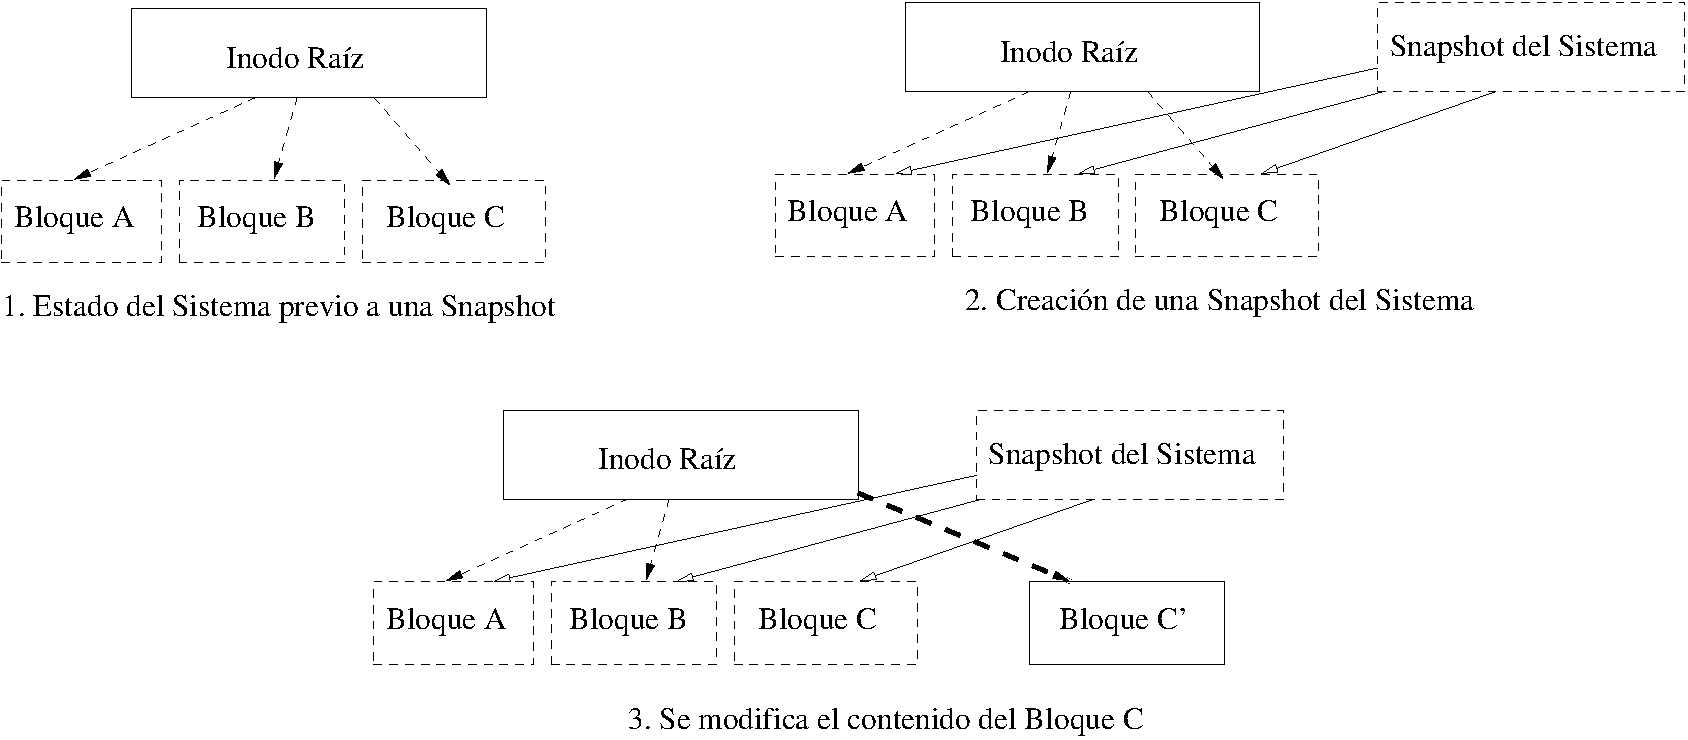
\includegraphics[width=1\linewidth]{figures/snapshots.pdf}
    \caption{Creación de una instantánea de un archivo}
    \label{fig:funcionamiento_snapshots}
\end{figure}

\begin{itemize}
    \item \textbf{Creación de la instantánea:}
        Partimos de un estado del sistema estable a partir del cual se crea la instantánea. Durante la creación de esta sobre un fichero, el sistema de ficheros captura el estado actual de los datos, generando una copia que refleja exactamente el contenido del mismo en ese instante, incluyendo todas las características de este, como su máscara UGO, propietario, entre otros.
    
    \item \textbf{Conservación de los datos originales:}
        Aunque el sistema puede continuar aceptando escrituras después de la creación de la instantánea, los datos originales permanecen intactos y accesibles a través de la misma. Es importante tener en cuenta que, aunque el sistema pueda seguir atendiendo peticiones de escritura después de crear una instantánea, la información salvaguardada en esta es una foto del estado del fichero o directorio en ese momento, pero su estado actual posiblemente habrá cambiado.
    
    \item \textbf{Restauración:}
        En situaciones de errores, pérdida de datos o cambios no deseados, es factible restaurar el fichero o directorio a un estado anterior utilizando la correspondiente instantánea. Esta restauración implica la vuelta del fichero o directorio a su estado capturado en el momento de la creación de la misma, incluyendo tanto su contenido como sus metadatos y configuraciones específicas.
        
\end{itemize}

Estas instantáneas se basan en la tecnología de copy on write (COW). A diferencia del COW utilizado para compartir memoria entre procesos diferentes, como por ejemplo a través de la llamada fork, esta implementación se emplea para compartir bloques de datos preexistentes al crear la instantánea. Solo se realiza una copia de los mismos cuando se modifican, optimizando así el proceso.

\subsection{Journaling en sistemas de ficheros de Linux}

El journaling, o registro de transacciones, es una técnica fundamental utilizada en los sistemas de ficheros para garantizar la integridad de los datos en caso de fallos del sistema o interrupciones inesperadas, como cortes de energía. Esta técnica consiste en mantener un registro detallado de las operaciones de escritura que se realizan en el sistema de ficheros antes de que se apliquen de manera definitiva \cite{bovet2005,linuxstorage}.

\begin{figure}[h!]
    \centering
    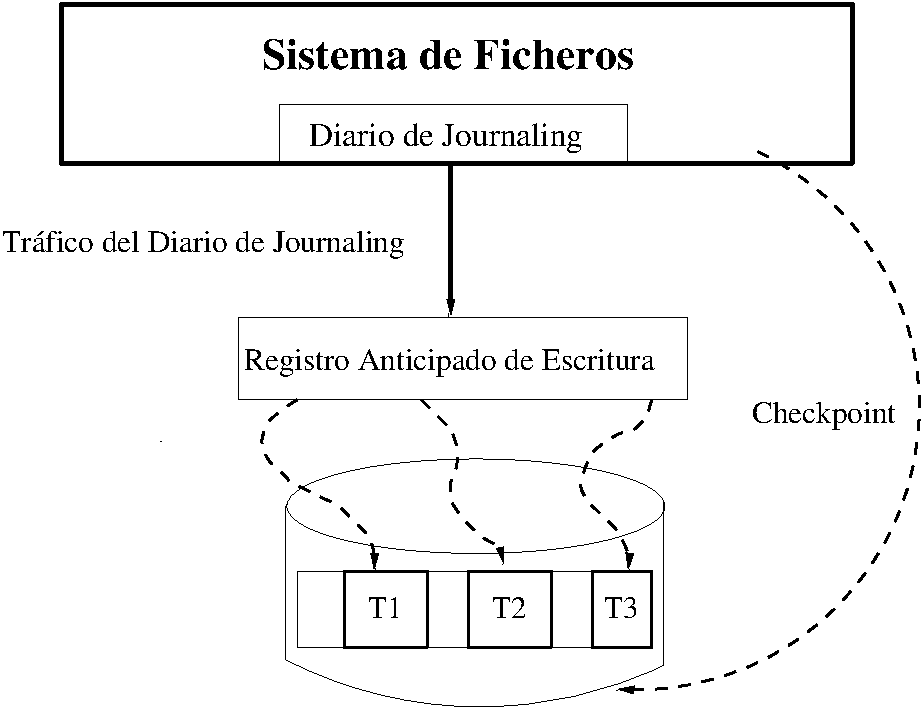
\includegraphics[width=0.55\linewidth]{figures/journaling.pdf}
    \caption{Ilustración del funcionamiento del journaling}
    \label{fig:funcionamiento_journaling}
\end{figure}

La gran mayoría de sistemas de ficheros dividen el proceso de journaling en tres pasos, que aparecen en la figura \ref{fig:funcionamiento_journaling} y se describen a continuación:

\begin{enumerate}
    \item \textbf{Registro inicial en el journal:} En esta etapa, se inicia el proceso creando una duplicación de los bloques destinados a ser escritos en el sistema de ficheros. Esta copia se almacena en el registro anticipado de escritura, y todos los datos registrados en esta fase quedan documentados en el diario de journaling del sistema de ficheros.

    \item \textbf{Confirmación en el journal:} Una vez que la transferencia de datos al registro anticipado de escritura se ha completado y los datos han sido confirmados en el diario de journaling, los bloques son finalmente escritos en el sistema de ficheros.

    \item \textbf{Finalización y confirmación en el sistema de ficheros:} En esta fase concluyente, después de finalizar la transferencia de datos al sistema de ficheros y confirmar la integridad en este último, se emite un checkpoint que valida el exitoso proceso de transferencia de datos. Posteriormente, las copias de los bloques almacenadas en el registro anticipado de escritura se descartan.
\end{enumerate}

El journaling también es beneficioso para minimizar la fragmentación y puede mejorar la eficiencia general del sistema de ficheros. Sin embargo, su objetivo principal es asegurar que las operaciones de escritura se completen de manera segura y coherente.

\subsection{Técnicas de gestión de los datos en discos: Trim y Defrag}

Dos técnicas clave sobresalen en la optimización del acceso a datos y el rendimiento eficiente: Trim y Defrag. Trim es esencial para maximizar tanto el rendimiento como la durabilidad de los dispositivos de estado sólido, siendo una técnica integrada en la gran mayoría de sistemas de ficheros actuales. Por otro lado, defrag se presenta como una técnica tradicional utilizada en discos duros magnéticos para organizar los datos y mejorar su accesibilidad, mediante la reorganización de los fragmentos de datos en el sistema de ficheros.

\subsubsection{Optimización de almacenamiento con Trim en SSD}

Trim es una técnica que capacita al sistema operativo para poder informar a una unidad de estado sólido basada en NAND flash acerca de los bloques de datos que ya no están en uso y pueden ser eliminados. Esta implementación no solo acelera la velocidad de escritura en los SSD, sino que también desempeña un papel clave en la prolongación de la vida útil de estos discos.\\

Cuando un fichero es eliminado de un SSD, el sistema operativo etiqueta esos bloques de memoria como "libres" para su posible sobreescritura. Sin embargo, en los SSD, la reescritura directa de bloques individuales, como en los discos duros magnéticos, no es posible. En cambio, los SSD deben borrar bloques completos antes de escribir nuevos datos. La función Trim mejora este proceso al enviar una señal al SSD, indicándole qué bloques de datos ya no están en uso. Esto permite que el SSD realice la "recolección de basura", donde los bloques marcados como no utilizados se borran y están listos para ser escritos nuevamente de manera más eficiente cuando sea necesario.

\subsubsection{Optimización de almacenamiento con Defrag en HDD}

La desfragmentación es una práctica esencial aplicada a los sistemas de ficheros modernos de discos duros magnéticos con el objetivo de reorganizar los fragmentos dispersos de datos en el disco. Este procedimiento tiene como finalidad mejorar el acceso a los archivos y, en última instancia, potenciar el rendimiento general del disco duro.\\

Es crucial resaltar que los discos duros magnéticos son especialmente susceptibles a la fragmentación debido a la naturaleza de su funcionamiento. En estos dispositivos, las pistas magnéticas en la superficie del disco almacenan información, y la cabeza de lectura/escritura debe desplazarse a lo largo de estas pistas para acceder a los datos.\\

Sin embargo, los SSD operan de manera completamente distinta, careciendo de cabezas de lectura/escritura móviles. En consecuencia, los SSD no experimentan los mismos problemas de fragmentación que los HDD y, por ende, no requieren procesos de desfragmentación tradicionales para mantener un rendimiento óptimo. La gestión de la fragmentación en los SSD está intrínsecamente integrada en su diseño y se aborda de manera más eficiente en comparación con los discos duros magnéticos.\\

Es importante destacar que la desfragmentación nunca ha sido una prioridad en los sistemas de ficheros de Linux, a diferencia de Windows, donde ha tenido una importancia significativa, especialmente en sistemas de ficheros como NTFS. En Windows, la desfragmentación se considera crucial para mantener el rendimiento del sistema. No obstante, en la actualidad, los sistemas de ficheros modernos de Linux, como ext4 y Btrfs, han comenzado a implementar técnicas de desfragmentación para mejorar la eficiencia del almacenamiento y el acceso a los datos. Estas mejoras reflejan un avance en la gestión del sistema de ficheros, adaptándose a las necesidades contemporáneas de los usuarios y a las capacidades de los dispositivos de almacenamiento modernos.

\subsection{Técnicas de gestión del espacio en disco: compresión y deduplicación}

Dos técnicas clave utilizadas por los sistemas de ficheros son la compresión y descompresión de archivos, así como la deduplicación. Estas estrategias juegan un papel vital en la eficiencia y la economía del almacenamiento digital, asegurando que aprovechemos al máximo nuestro espacio y recursos.

\subsubsection{Deduplicación de los datos}

La función de deduplicación se centra en eliminar duplicados exactos de datos, evitando la redundancia y mejorando la eficiencia en el almacenamiento. Generalmente los sistemas de ficheros abordan este proceso de la siguiente forma:

\begin{enumerate}
    \item \textbf{Identificación de datos duplicados:}
        El sistema de ficheros analiza constantemente los bloques de datos almacenados para identificar duplicados exactos. Esto puede aplicarse a nivel de ficheros completos o a bloques de datos más pequeños, según la implementación específica.
    
    \item \textbf{Creación de punteros compartidos:}
        En lugar de almacenar múltiples copias idénticas de un conjunto de datos, la deduplicación crea punteros compartidos que apuntan al mismo bloque de datos. Esto significa que, en la práctica, solo se guarda una copia de los datos duplicados, reduciendo el espacio necesario en disco.
    
    \item \textbf{Modos y configuración de deduplicación:}
        Algunos sistemas de ficheros permiten la deduplicación en tiempo real durante la escritura de datos. Otros también ofrecen opciones programadas, ejecutando el proceso en momentos específicos para minimizar el impacto en el rendimiento. Además, se puede configurar la deduplicación con políticas personalizadas, como la frecuencia de ejecución del proceso y las áreas particulares del sistema de ficheros que deben ser consideradas.
\end{enumerate}

La deduplicación de datos ofrece beneficios significativos en términos de ahorro de espacio en disco, especialmente en situaciones donde hay datos duplicados o redundantes. Sin embargo, es esencial considerar cuidadosamente la implementación y configuración de esta característica para maximizar sus beneficios sin comprometer el rendimiento del sistema.

\subsubsection{Compresión y descompresión de datos en sistemas de ficheros de Linux}

La compresión y descompresión de datos son procesos esenciales para optimizar el espacio en disco y mejorar la eficiencia en el almacenamiento. A continuación, al igual que con la deduplicación, detallaremos la implementación general que siguen los sistemas de ficheros para abordar esta técnica:

\begin{itemize}
    \item \textbf{Compresión en tiempo real:}
    Este enfoque implica la compresión de datos durante la escritura en el sistema de ficheros. Los datos son comprimidos antes de ser almacenados en el disco, lo que proporciona ahorros inmediatos en espacio. Sin embargo, puede haber un ligero impacto en el rendimiento durante la escritura debido al procesamiento adicional de compresión.
    
    \item \textbf{Compresión programada o por lotes:}
    En algunos casos, la compresión se programa para ejecutarse en momentos específicos o como un proceso por lotes. Esta estrategia permite realizar la compresión cuando la carga del sistema es menor, minimizando el impacto en el rendimiento. La compresión por lotes puede aplicarse a ficheros individuales o a directorios completos, empaquetando y comprimiendo la información según sea necesario. 
\end{itemize}

\subsection{Encriptación y seguridad en sistemas de ficheros}

La seguridad de los datos es una preocupación creciente en la era digital, especialmente en entornos donde la integridad y confidencialidad de la información son críticas. Los sistemas de ficheros EXT4, BTRFS, XFS y ZFS ofrecen diversas características de seguridad, incluyendo encriptación y mecanismos de protección avanzados que los hacen adecuados para entornos que manejan datos sensibles.

\subsubsection{Encriptación de datos}

La encriptación en el nivel de sistema de ficheros permite asegurar que los datos almacenados en disco sean inaccesibles sin las credenciales adecuadas. Mientras que EXT4 no cuenta con soporte nativo para encriptación, soluciones como eCryptfs y Fscrypt permiten añadir una capa de encriptación sobre este sistema de ficheros.\\

Por otro lado, BTRFS y ZFS integran capacidades de encriptación nativa que facilitan la gestión segura de los datos sin la necesidad de herramientas adicionales. ZFS ofrece encriptación nativa desde su versión 0.8, permitiendo la encriptación de datos y metadatos de manera transparente para el usuario. BTRFS también soporta encriptación a través de configuraciones específicas del kernel.

\subsubsection{Protección contra manipulaciones y corrupción de datos}

Además de la encriptación, la integridad de datos es otro pilar fundamental de la seguridad en sistemas de ficheros. ZFS destaca en este aspecto con su diseño que utiliza sumas de comprobación para todos los bloques de datos, lo que permite detectar y corregir errores automáticamente. BTRFS proporciona características similares con su enfoque en la redundancia y la capacidad de reparar datos corruptos utilizando copias almacenadas.\\

XFS y EXT4, mientras tanto, ofrecen opciones de journaling que mejoran la resistencia del sistema de ficheros frente a fallos del sistema, garantizando que las operaciones de ficheros se completen correctamente o se reviertan en caso de interrupción.

\subsection{Resumen de las características en los sistemas de ficheros a analizar}

\begin{table}[h!]
\centering
\caption{Comparación de características de los sistemas de ficheros EXT4, BTRFS, XFS y ZFS}
\label{tab:comparative-features}
\resizebox{\textwidth}{!}{%
\begin{tabular}{|l|c|c|c|c|}
\hline
\textbf{Característica} & \textbf{EXT4} & \textbf{BTRFS} & \textbf{XFS} & \textbf{ZFS} \\ \hline
Journaling & \checkmark & \checkmark & \checkmark & \checkmark \\ \hline
Snapshots & $\times$ & \checkmark & $\times$ & \checkmark \\ \hline
Deduplicación & $\times$ & \checkmark & $\times$ & \checkmark \\ \hline
Compresión & $\times$ & \checkmark & $\times$ & \checkmark \\ \hline
Integridad de datos & \checkmark & \checkmark & \checkmark & \checkmark \\ \hline
Cachés del sistema & \checkmark & \checkmark & \checkmark & \checkmark \\ \hline
Copy on Write (COW) & $\times$ & \checkmark & $\times$ & \checkmark \\ \hline
Tamaño de bloque & \texttt{1KiB-64KiB} & \texttt{4KiB-64KiB} & \texttt{512B-64KiB} & \texttt{4KiB-128KiB} \\ \hline
Tamaño nombre de archivo & \texttt{255 bytes} & \texttt{255 bytes} & \texttt{255 bytes} & \texttt{255 bytes} \\ \hline
Encriptación & \texttt{eCryptfs/Fscrypt} & \texttt{Kernel} & $\times$ & \checkmark \\ \hline
Protección de datos & \texttt{Journaling} & \texttt{Checksum} & \texttt{Journaling} & \texttt{Checksum} \\ \hline
TRIM Support & \checkmark & \checkmark & $\times$ & \checkmark \\ \hline
Defragmentación & \checkmark & $\times$ & \checkmark & $\times$ \\ \hline
\end{tabular}
}
\end{table}




